\section{Results and discussion}\label{sec:results}

To serve as a baseline, a pipeline was trained using synthetic FOREST as the source domain and their artificially degraded version as the target domain. 
To obtain such data, the degradation model described in \ref{subsec:baseline_degradation_model} was applied, blurring and adding noise to the synthetic FOREST images.
This degradation model is stochastic, but with unknown parameters. The objective is to observe how the pipeline is able to mimic the degradation model used in the target domain.On the other side, the main pipeline was trained using synthetic FOREST as the source domain and real FOREST as the target domain. 
In this case, the degradation model is unknown and the objective is to observe how the pipeline is able to estimate it, generating LR versions of the synthetic FOREST images that come from the same distribution as the real FOREST images.

    \subsection{Source domain}

        This subsection will show the results from the experiments performed on the source domain.
        The process consists of degrading the synthetic HR FOREST images using the generator trained using adversarial learning and then super resolving it using the corresponding SR model used in the pipeline.
        This is the equivalent of the black arrows flow describes in fig. \ref{fig:3-GAN-degradation-model}. 

        As in this case the ground truth is known, the performance of the SR model can be evaluated using metrics like PSNR and SSIM. 
        Unfortunately, as the target and the source domain are not paired, the effects of the degradation model have to be evaluated using alternative methods.

        Fig. \ref{fig:5-source_domain_sample} shows the results of both pipelines when applied to one sample from the source domain. 
        For comparison, a simple gaussian blurring + downscaling is also shown. 
        The main differences can be seen on the degraded LR images. While the baseline pipeline produces images very similar to gaussian blurring + downscaling, 
        the adapted pipeline produces much more blurry images with more noise, suggesting that FOREST-2 produces less resolution than what was initially expected. 
        However, both super resolved images yield better performance than just using bicubic interpolation, and they are very similar between them.
        This suggests that the super resolution model is able to recover the details lost during stronger degradation processes, but there seems to be a limit to the amount of detail that can be recovered. 
        Even though the starting point is different ( baseline LR is less blurry than adapted LR), the final result is very similar.

        The estimated kernel and noise for both pipelines is also shown in fig. \ref{fig:5-source_domain_sample}. 
        While the baseline kernel is very simple and the noise is more or less uniform across the image, the adapted kernel is more complex and the noise seems to be strongly correlated with the image intensity.
        It is important not to overinterpret this result, as the kernel and noise are estimated using overparametrized models, and multiple combinations of kernel and noise may produce similar results. 
        However, it is interesting to see that the adapted pipeline is able to estimate a more complex degradation model, which is closer to the real degradation model used in the target domain.

        \begin{figure}[H]
            \centering
            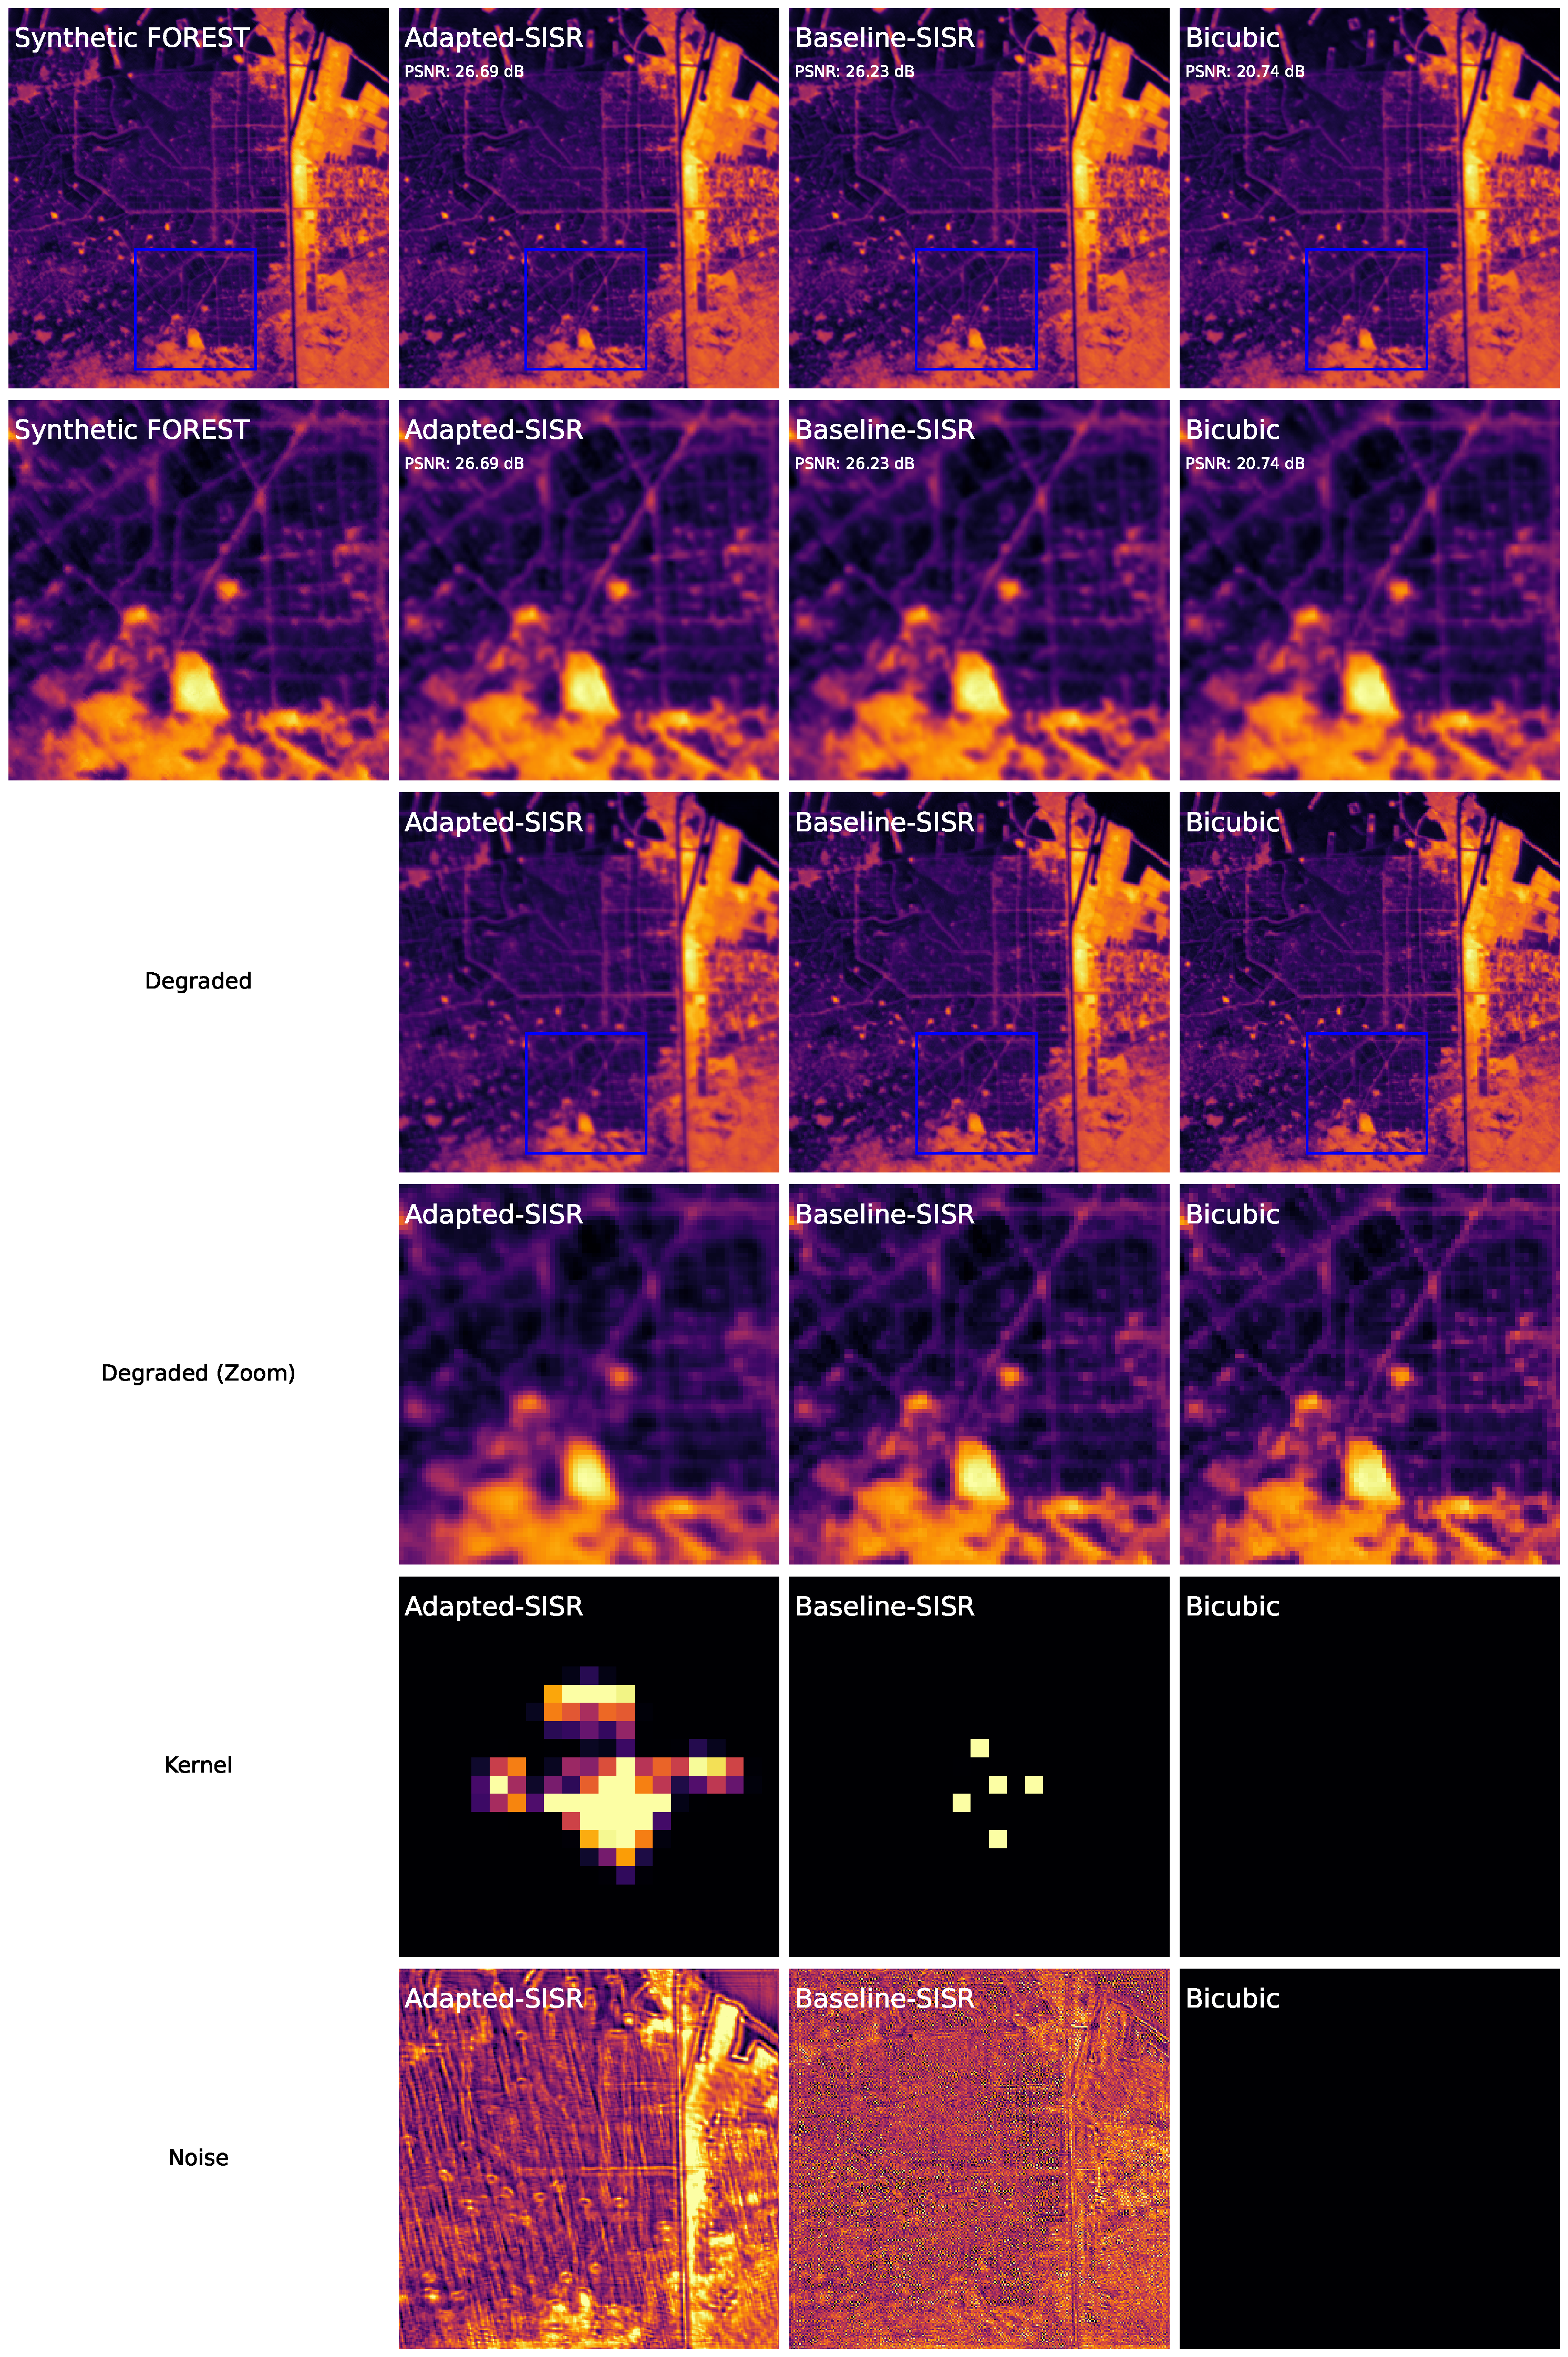
\includegraphics[width=\textwidth]{Includes/5-source_prediction-sample.pdf}
            \caption{Applying different degradation models on an HR sample. 
                    In the Baseline SISR, the target domain used for training the generator is composed of sysnthetic HR FOREST-2 images degraded using the model detailed in \ref{subsec:baseline_degradation_model}.
                    In the adapted SISR, the target domain used for training the generator is composed of real FOREST-2 images.}
            \label{fig:5-source_domain_sample}
        \end{figure}
        \pagebreak

        \subsubsection{Effects of the degradation model}

        Fig. \ref{fig:5-source-domain-comparison} shows the performance obtained by super resolving the degraded synthetic FOREST images for the whole validation dataset.
        In the upper row (a), the corresponding model is used to obtain the super resolved images. 
        The performance, both in PSNR and SSIM, are very similar for both pipelines. The LPIPS shows a consistent behavior too.
        In the lower row (b), a simple bicubic interpolation is used to super resolve the degraded images. 
        In this case, the baseline LR version yields better results than the adapted LR version, both in PSNR and SSIM.
        This suggests that the learned degradation model from FOREST-2 images loses more information than the baseline, resulting in a lower ground sampling distance than what is expected.
        Interestingly, the SR model is able to recover a big portion of the information, as the performance after using the SR models is very similar. 
        This shows the relevance of the domain gap in super resolution, the SR model is able to apply the inverse of the degradation function in most cases, and the problem relies on that in the most common experiments, the wrong degradation model is shown to the model. 
        Moreover, the LPIPS for the adapted LR version is better than the baseline LR version. FADSPOFKDASOFADOJSFJOADOJFAD

        \begin{figure}[H]
            \centering
            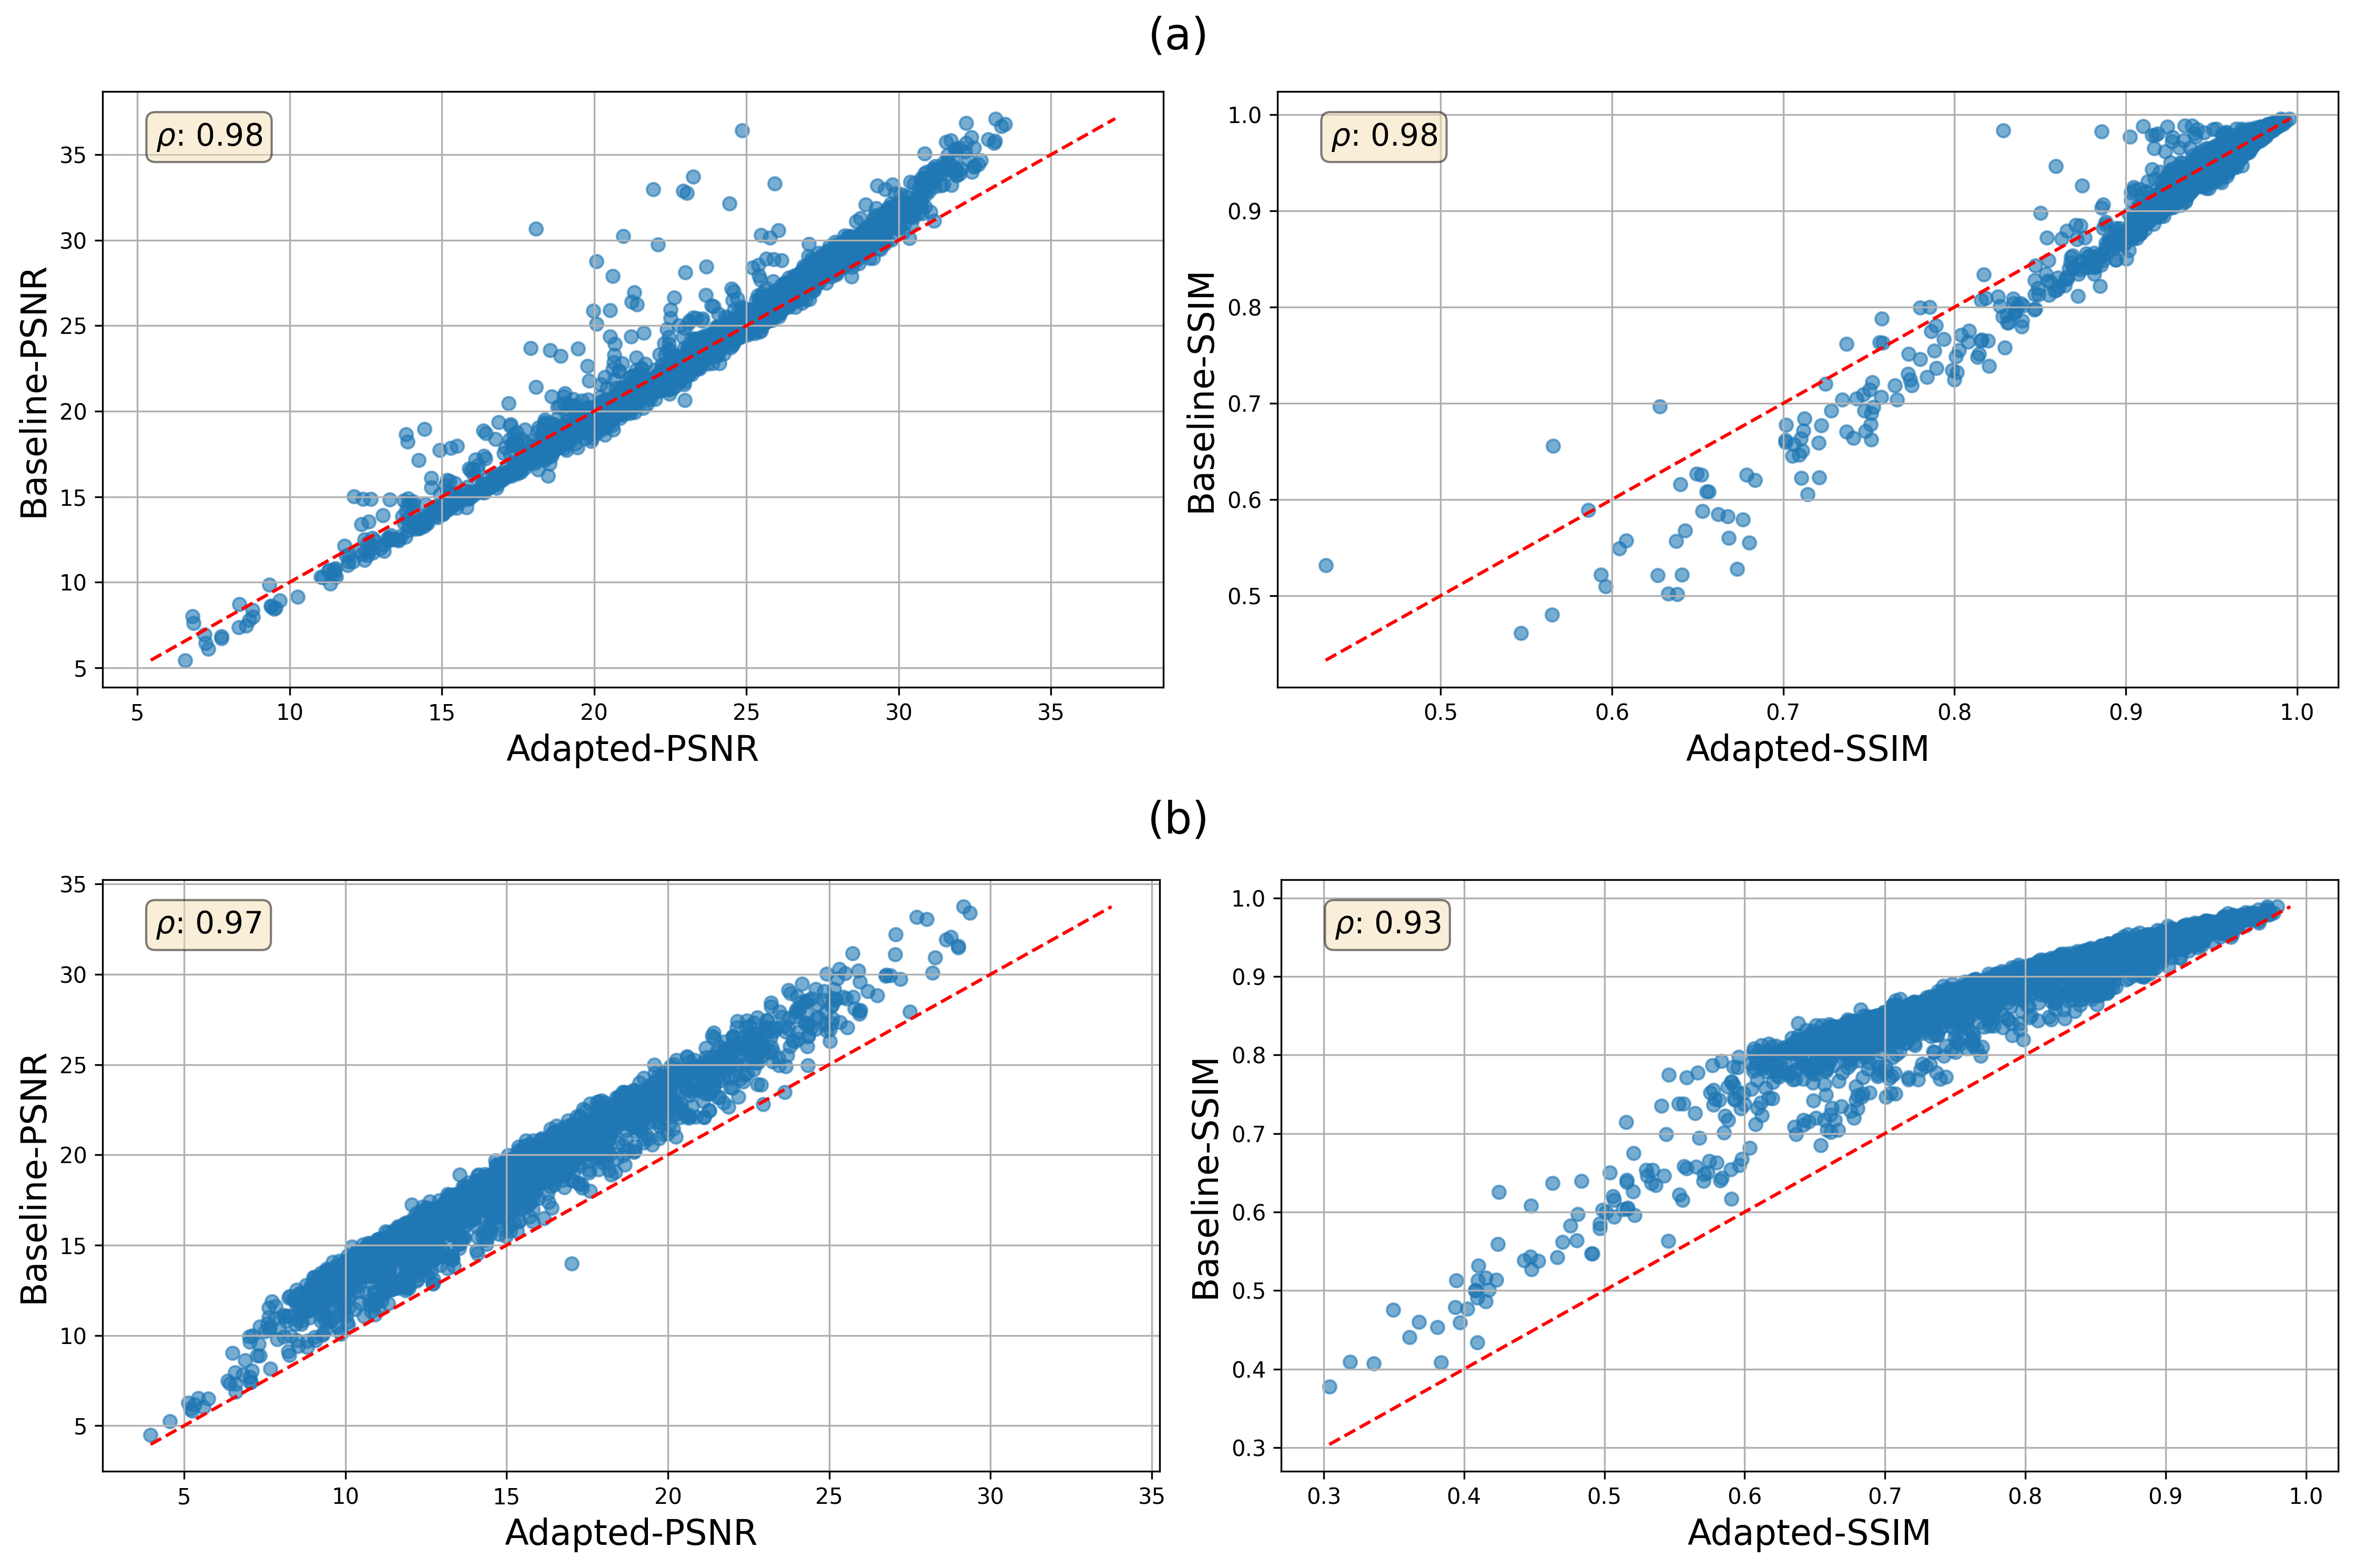
\includegraphics[width=\textwidth]{Includes/5-source-domain-comparison.png}
            \caption{Performance obtained by super resolving the degraded synthetic FOREST images. 
                        In (a), the correspondingly trained SISR model is applied. 
                        In (b), a simple bicubic interpolation is used to super resolve the degraded images. }
            \label{fig:5-source-domain-comparison}
        \end{figure}

        An alternative way to evaluate the lost frequency components due to the degradation model is by analyzing the frequency domain of the LR images.
        An example of the analysis of the whole validation dataset is shown in Fig. \ref{fig:5-lr-images-fft-comparison}. 
        In (a) the log magnitude of the FFT is across different spatial frequency values for the different degraded images is displayed. 
        The spatial frequency is obtained from the radial distance to the center of the FFT, as shown in \ref{subsubsec:frequency_domain_analysis}.
        In (b), the amplification with respect to a simple gaussian blurring + downscaling is shown. 
        While the baseline does not lose much information with respect to gaussian blurring + downscaling, the adapted pipeline consistently diminishes high frequency components starting at 0.1 cycles per pixel. 
        It is important to note that 0.1 cycles per pixel at a 210m GSD corresponds to a cycle frequency of 21m.
        These results are consistent with the observations noted in Fig. \ref{fig:5-source-domain-comparison}, where the adapted pipeline yields worse LR images.
    
        \begin{figure}[H]
            \centering
            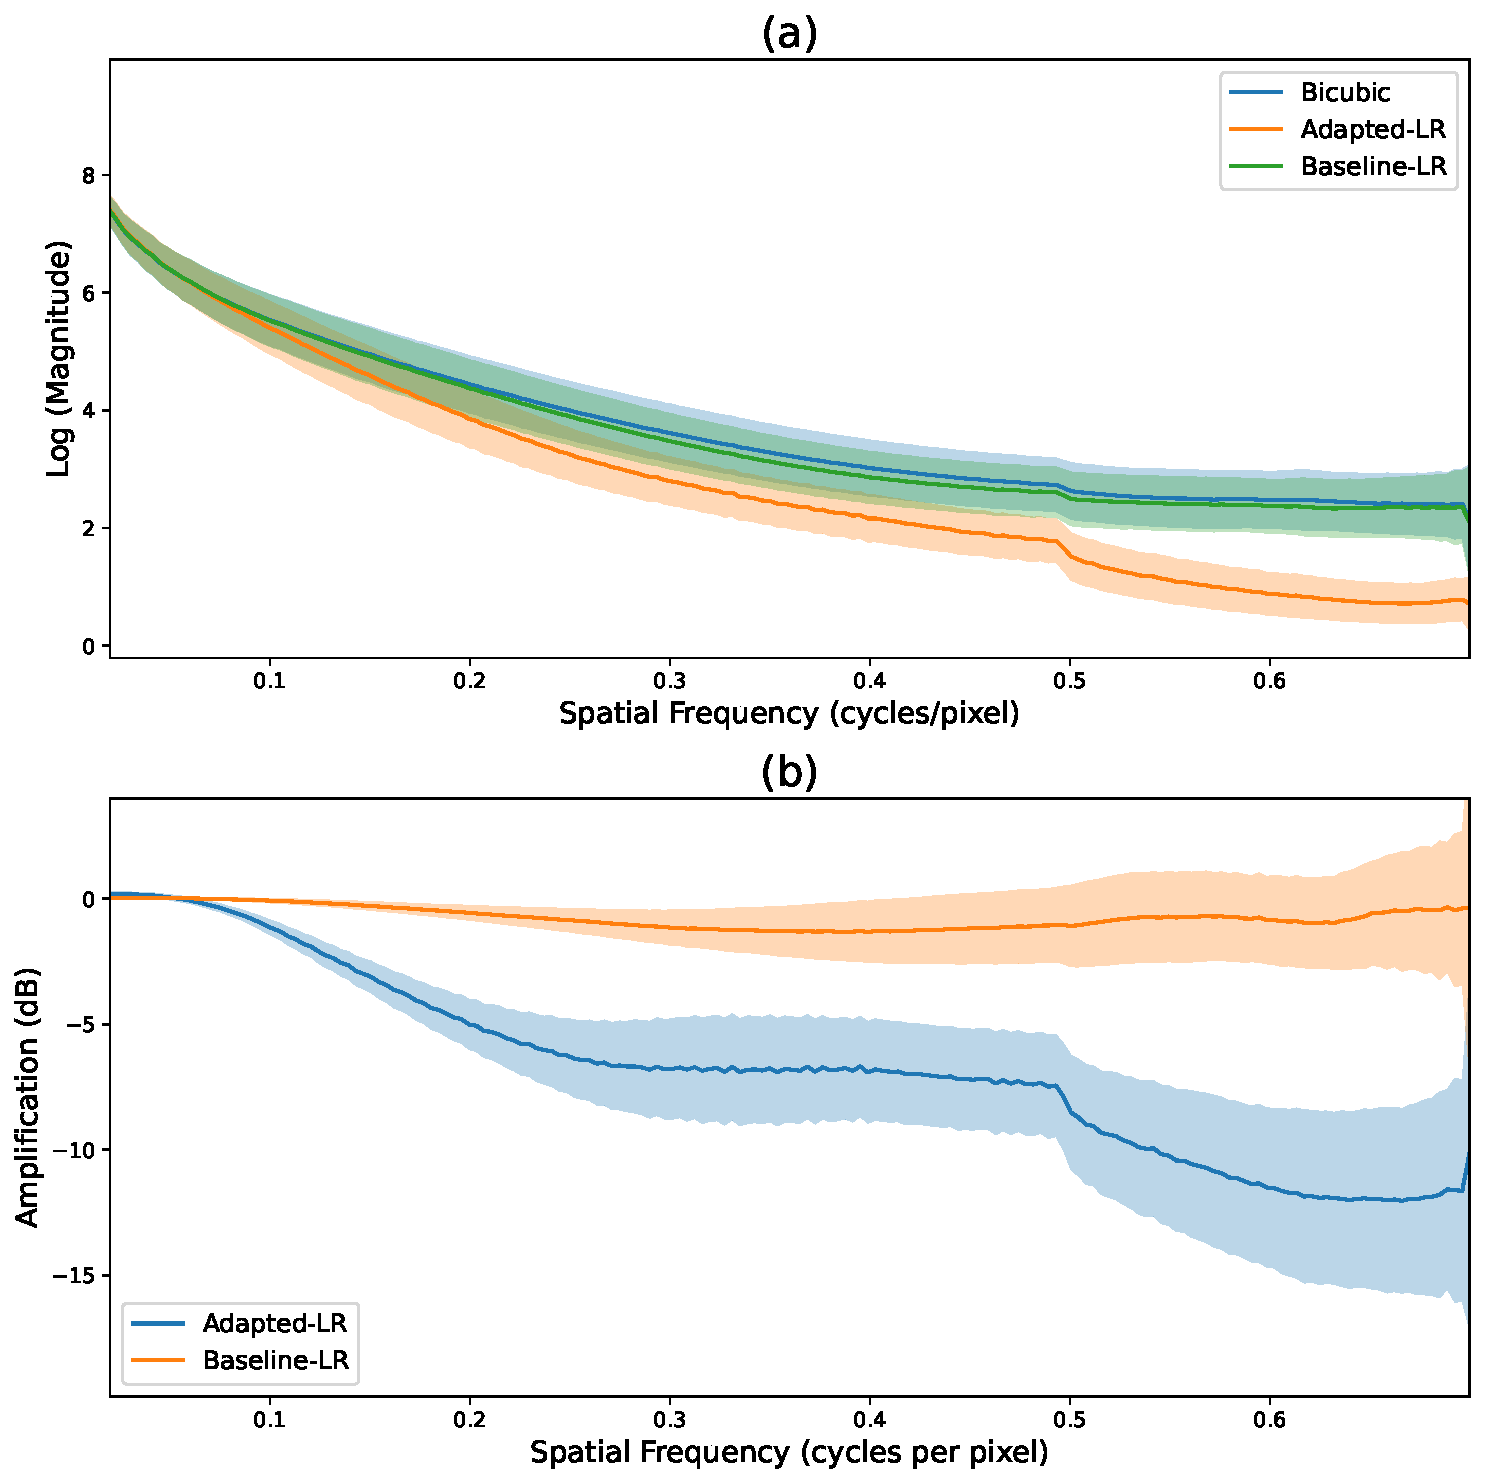
\includegraphics[scale=0.5]{Includes/5-source-lr-amplification-statistics.pdf}
            \caption{Frequency domain analysis of the LR images obtained by applying different degradation models on the HR sample displayed in Fig. \ref{fig:5-source_domain_sample}.
                     In (a), the log of the magnitude of the FFT for the LR images is shown,
                     while in (b), the amplification with respect to a  simple gaussian blurring + downscaling is shown.}
            \label{fig:5-lr-images-fft-comparison}
        \end{figure}

    \pagebreak

        
            
    
    \subsection{Target domain}

        This subsection will show the results from the experiments performed on the target domain, this is the equivalent of the red arrows flow describes in fig. \ref{fig:3-GAN-degradation-model}.
        In this case, the GAN trained for the degradation model is discarded and only the super resolution model is used.
        The input images are real FOREST-2 images, and the output images are super resolved versions of them. 
        Due to the unpaired nature of the dataset, the performance of the SR model can not be evaluated using metrics like PSNR and SSIM. 
        Other alternatives will be presented, and a qualitative analysis will be performed. 
        Additionally, a quantitative analysis will be discussed using a very small sample of paired data obtained by synchronizing the overpass of FOREST-2 with the route of ECOSTRESS.


        In Fig. \ref{fig:5-target_prediction_sample}, the super resolutions models were used with a 264x264 pixels crop of a real FOREST-2 image.

    

        \begin{figure}[H]
            \centering
            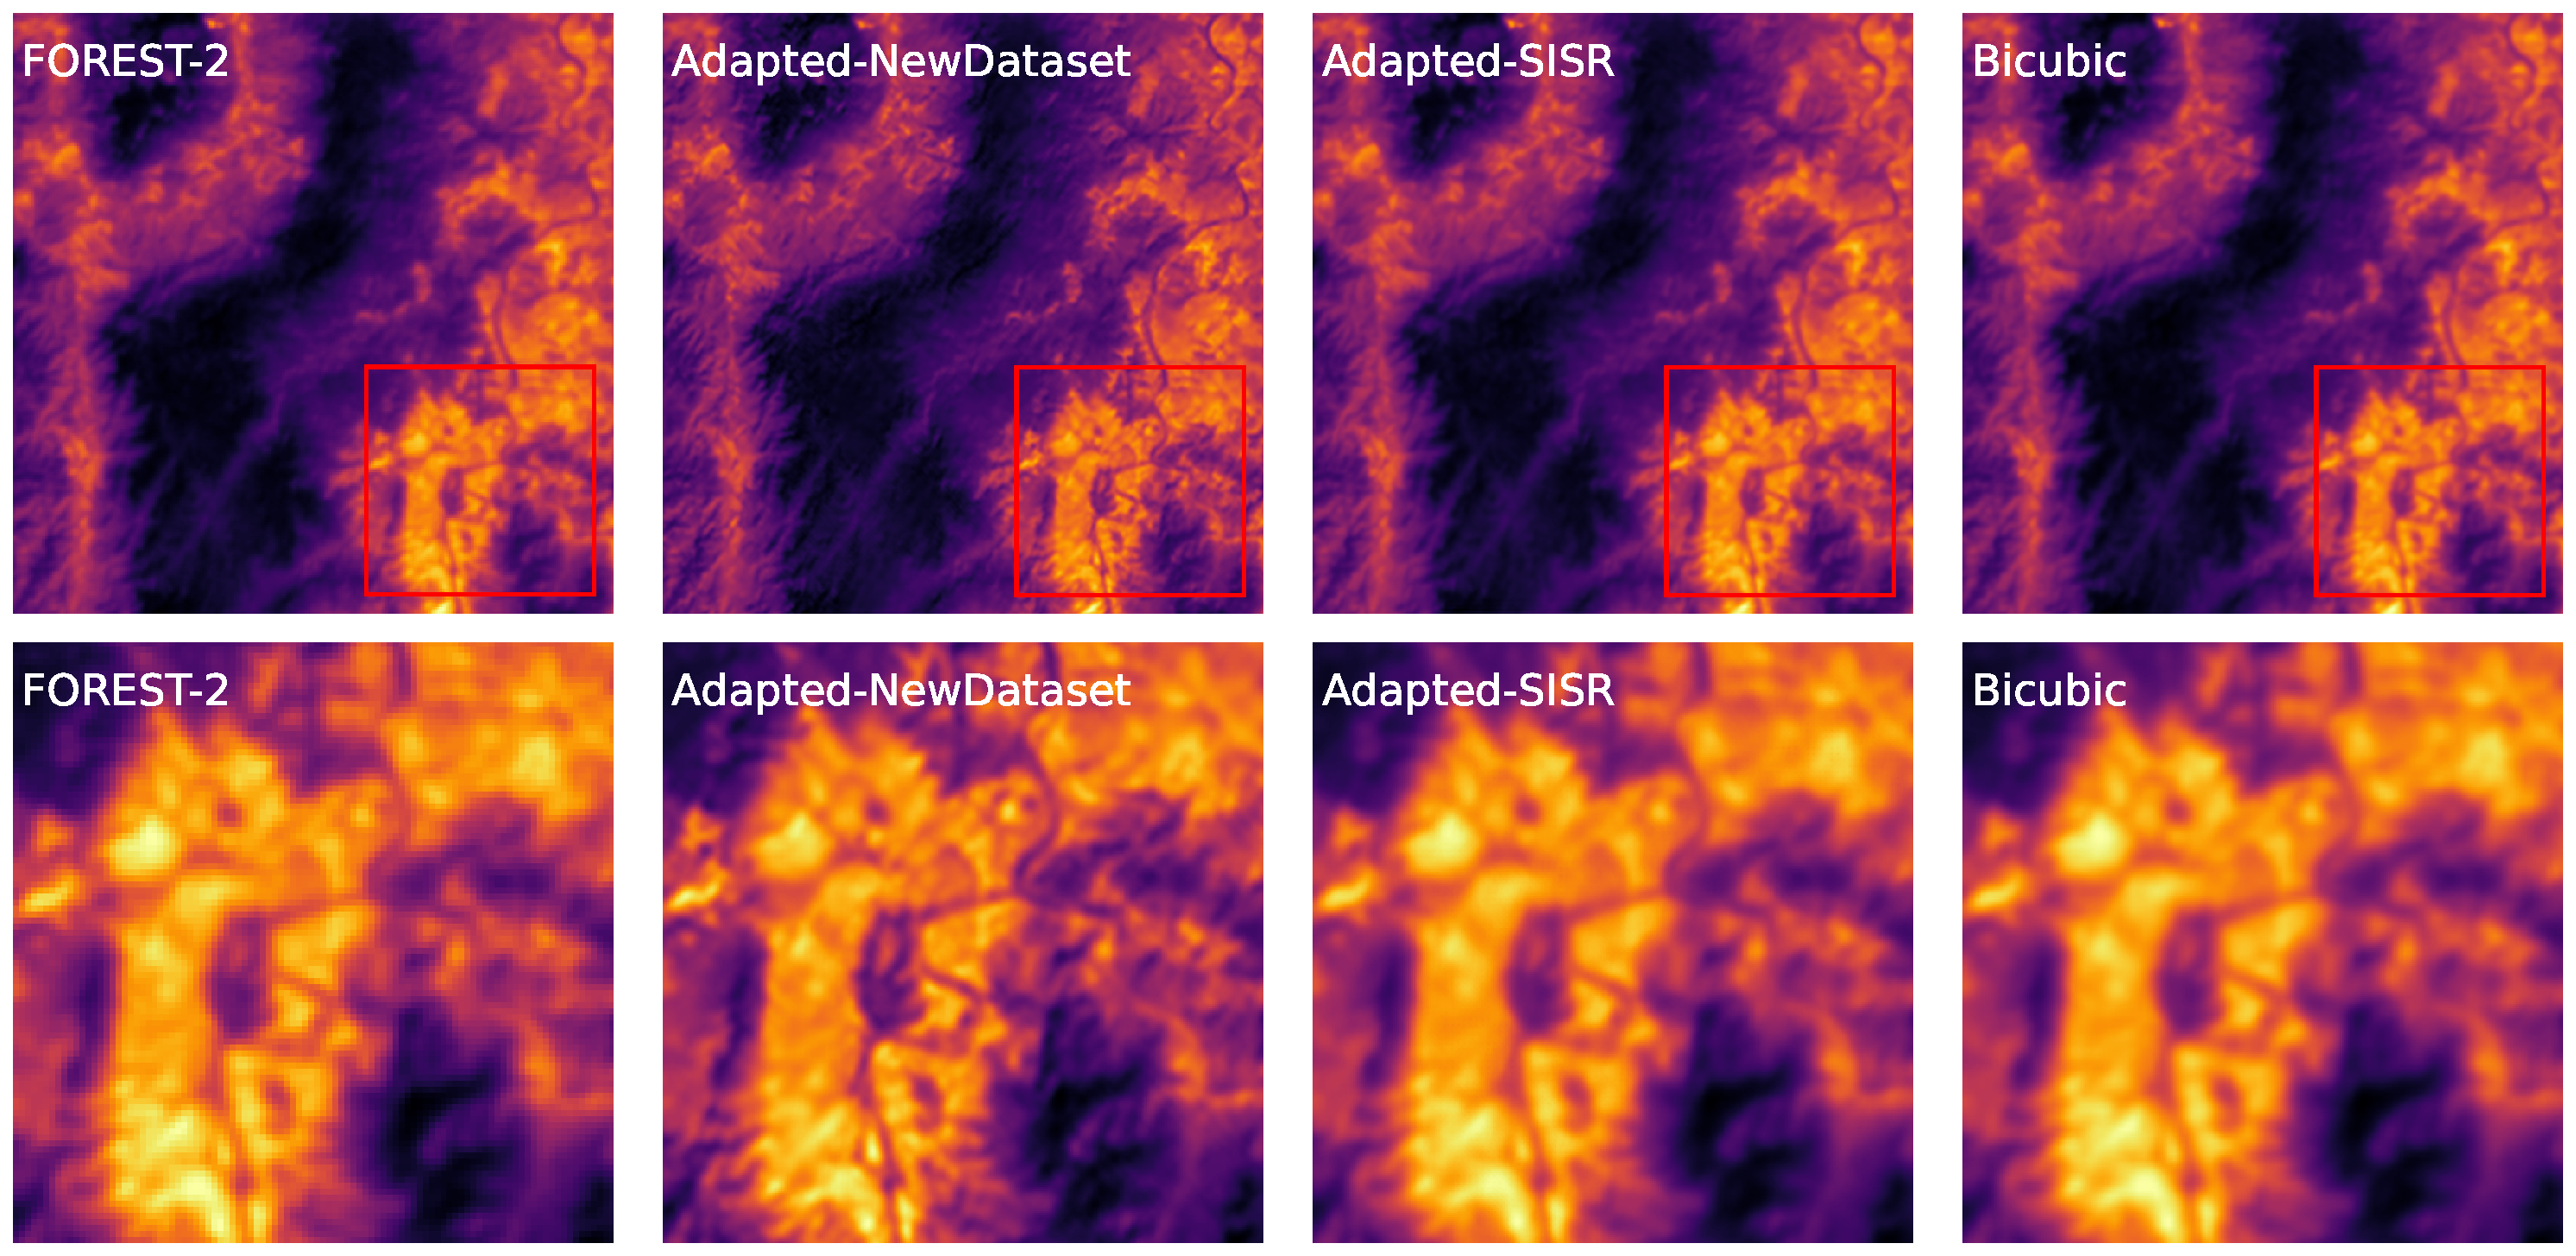
\includegraphics[scale=0.28]{Includes/5-target_prediction_sample.pdf}
            \caption{Super Resolved Forest-2 Scene using different SR models.
                     In the upper row, the image is displayed. A detailed zoom is displayed below}
            \label{fig:5-target_prediction_sample}
        \end{figure}


        \begin{figure}[H]
            \centering
            \includegraphics[scale=0.28]{Includes/6-target-fft-sample.pdf}
            \caption{Super Resolved Forest-2 Scene using different SR models. 
                     In the upper row, the image is displayed. The log magnitude of the FFT is displayed below.}
            \label{fig:6-target-fft-sample}
        \end{figure}


        \begin{figure}[H]
            \centering
            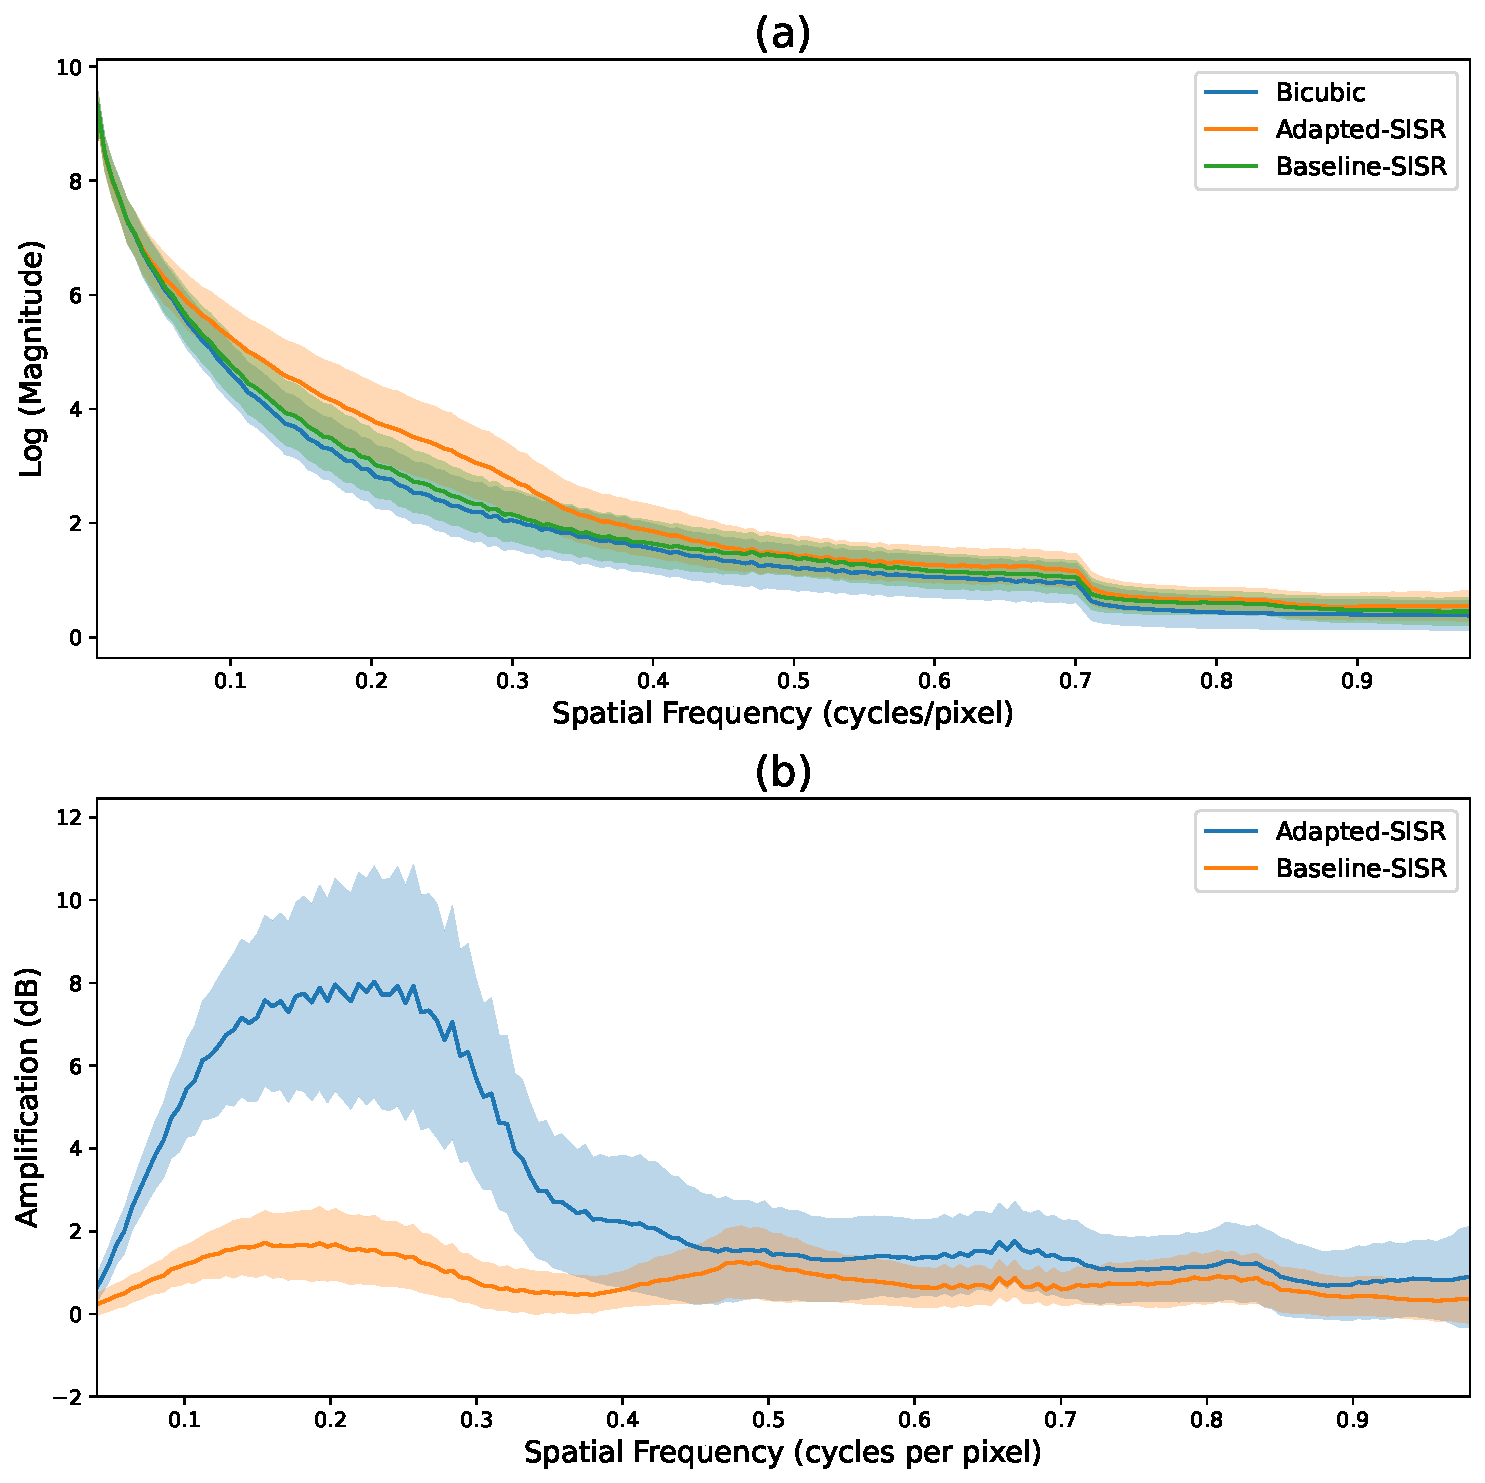
\includegraphics[scale=0.5]{Includes/5-target-amplification-statistics.pdf}
            \caption{Frequency domain analysis of the SR images obtained by applying different SR models to the real FOREST-2 validation dataset.
            In (a), the log of the magnitude of the FFT for the SR images is shown,
            while in (b), the amplification with respect to a  simple bicubic upsampling is displayed.}
            \label{fig:5-target-amplification-statistics}
        \end{figure}

        \begin{figure}[H]
            \centering
            \includegraphics[scale=0.28]{Includes/6-target-gradient-analysis-image.pdf}
            \caption{Gradient analysis of the super resolved images using different SR models for scenes coming from the real FOREST-2 validation dataset.
                     In the upper row, the image is displayed. The gradients in the x and y direction ($G_x$ and $G_y$ respectiely) are displayed below.
                     the gradient magnitude $|G|$ is displayed in the bottom row.}
            \label{fig:6-target-gradient-analysis-image}
        \end{figure}

        \begin{figure}[H]
            \centering
            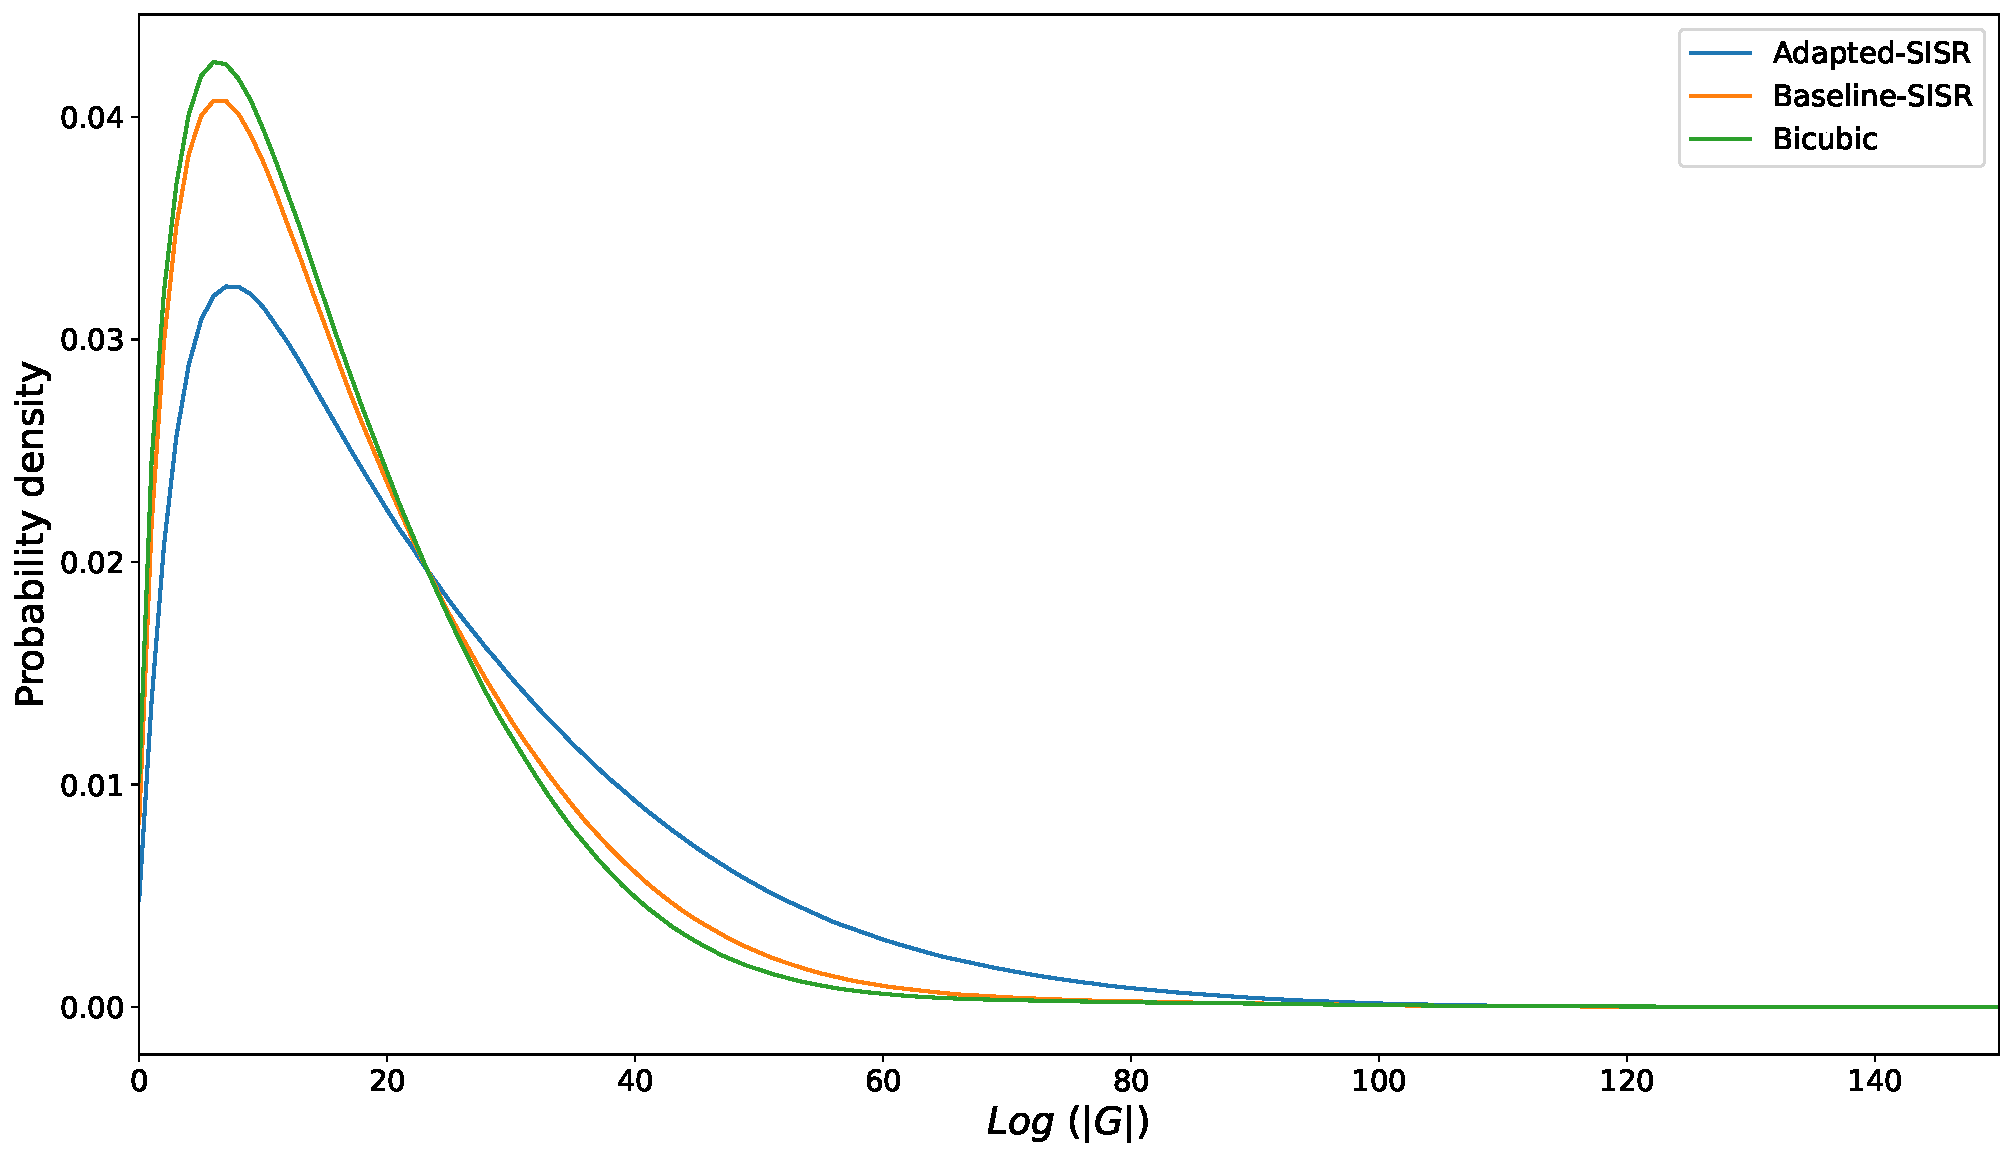
\includegraphics[scale=0.4]{Includes/5-gradient-histogram-validation-dataset.pdf}
            \caption{Histogram of the gradient magnitude $|G|$ for the whole validation real FOREST-2 dataset.}
            \label{fig:5-gradient-histogram-validation-dataset}
        \end{figure}

    \subsection{Effects of the domain gap}

        The combination of the probabilistic degradation model and the SR model were proven helpful to bridge the domain gap between the source and the target domain.
        However, it is important to understand what happens when the target domain used in training does not match the conditions that will occur in the real world.
        Two situations are identified, the first one is when the target domain used in training is more complex than what will be used in production, and the second one is when the target domain used in training is simpler than what will be used in production.
        The latter was largely adressed in this work, when the HR-LR pairs are generated using a baseline degradation model, which is overly optimistic. 
        Another example of it would be that images taken from FOREST-2 in several years may not have the same distribution as current images, as the instruments may have degraded over time.
        However, the first one was not addressed, and is the focus of this subsection.
        
        To simulate this situation, the model trained using real FOREST-2 images was used to super resolve synthetic FOREST images degraded using the baseline degradation model.
        The results are shown in Figs. \ref{fig:5-target-prediction-with-domain-gap} and \ref{fig:5-target-prediction-with-domain-gap-fft}.
        The performance of the adapted model is catastrophic, producing several artifacts and yielding a PSNR difference of approximately 10dB, which represent a 10x difference in terms of MSE.

        \begin{figure}[H]
            \centering
            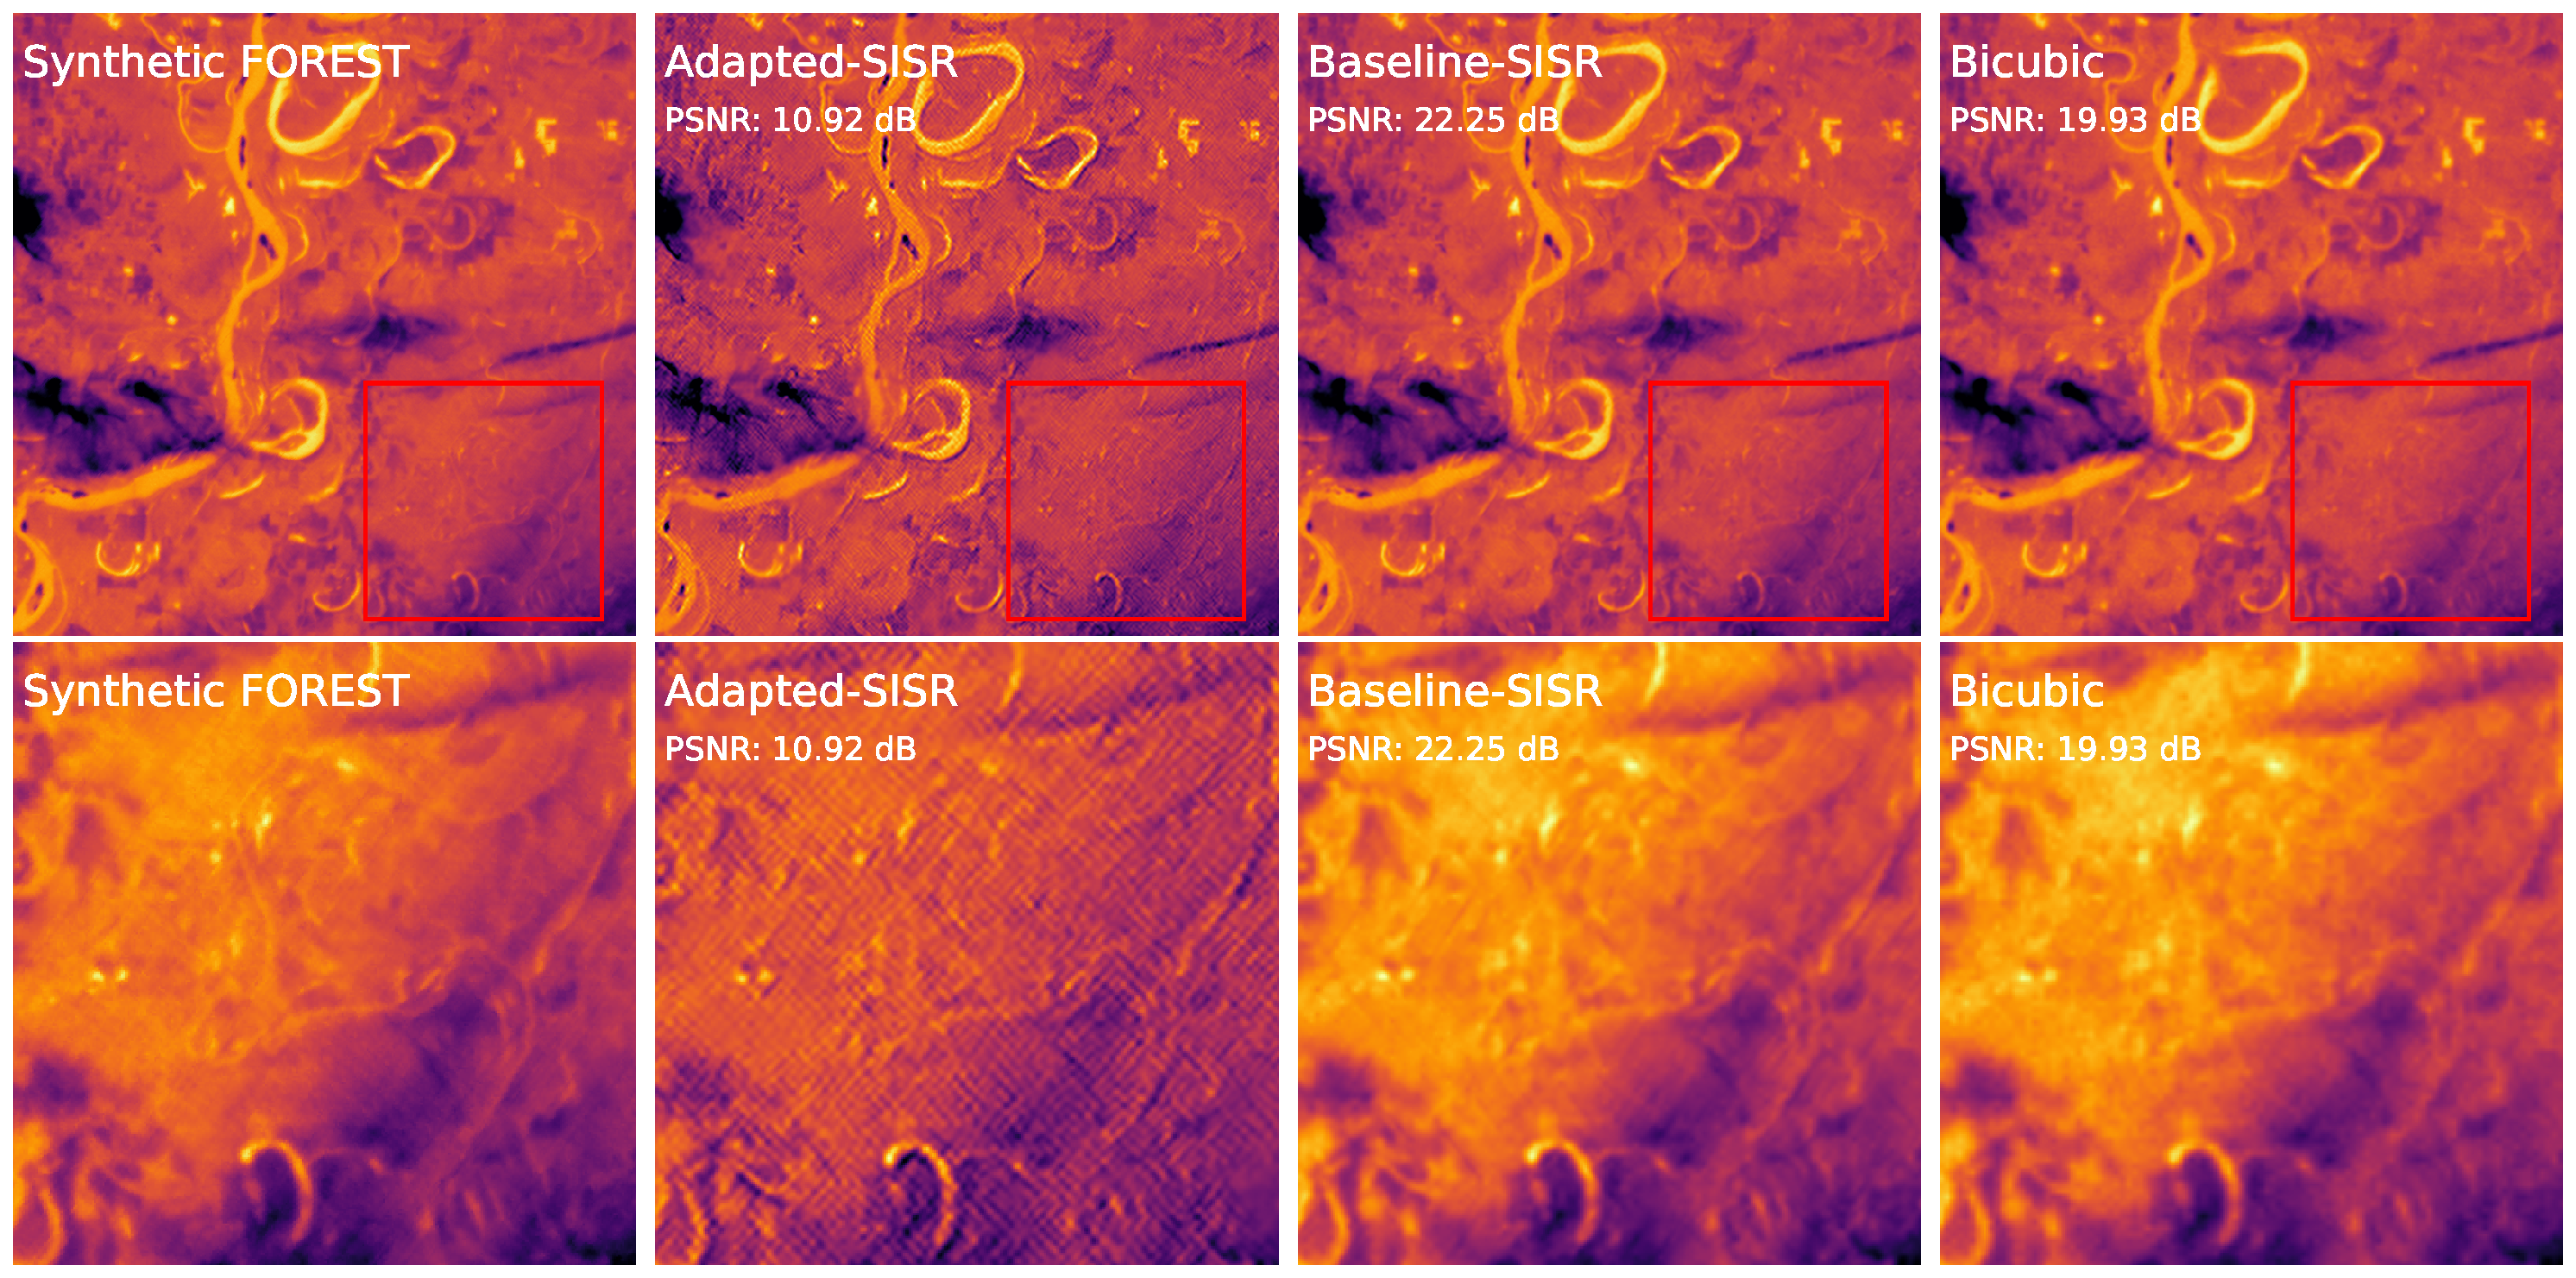
\includegraphics[scale=0.28]{Includes/5-target-prediction-with-domain-gap.pdf}
            \caption{Effects of using a model trained with on different domain than at inference time. 
                     When using an Synthetic FOREST image degraded with the baseline degradation model as an input, the model trained using real FOREST-2 data as the target domain generates several artifacts and underperforms severly in terms of PSNR. }
            \label{fig:5-target-prediction-with-domain-gap}
        \end{figure}

        The performance results in terms of different metrics are shown in Fig. \ref{fig:5-target-prediction-with-domain-gap-dataset}. 
        In the conditions described above, the adapted super resolution model underperforms severly considered metric.


        \begin{figure}[H]
            \centering
            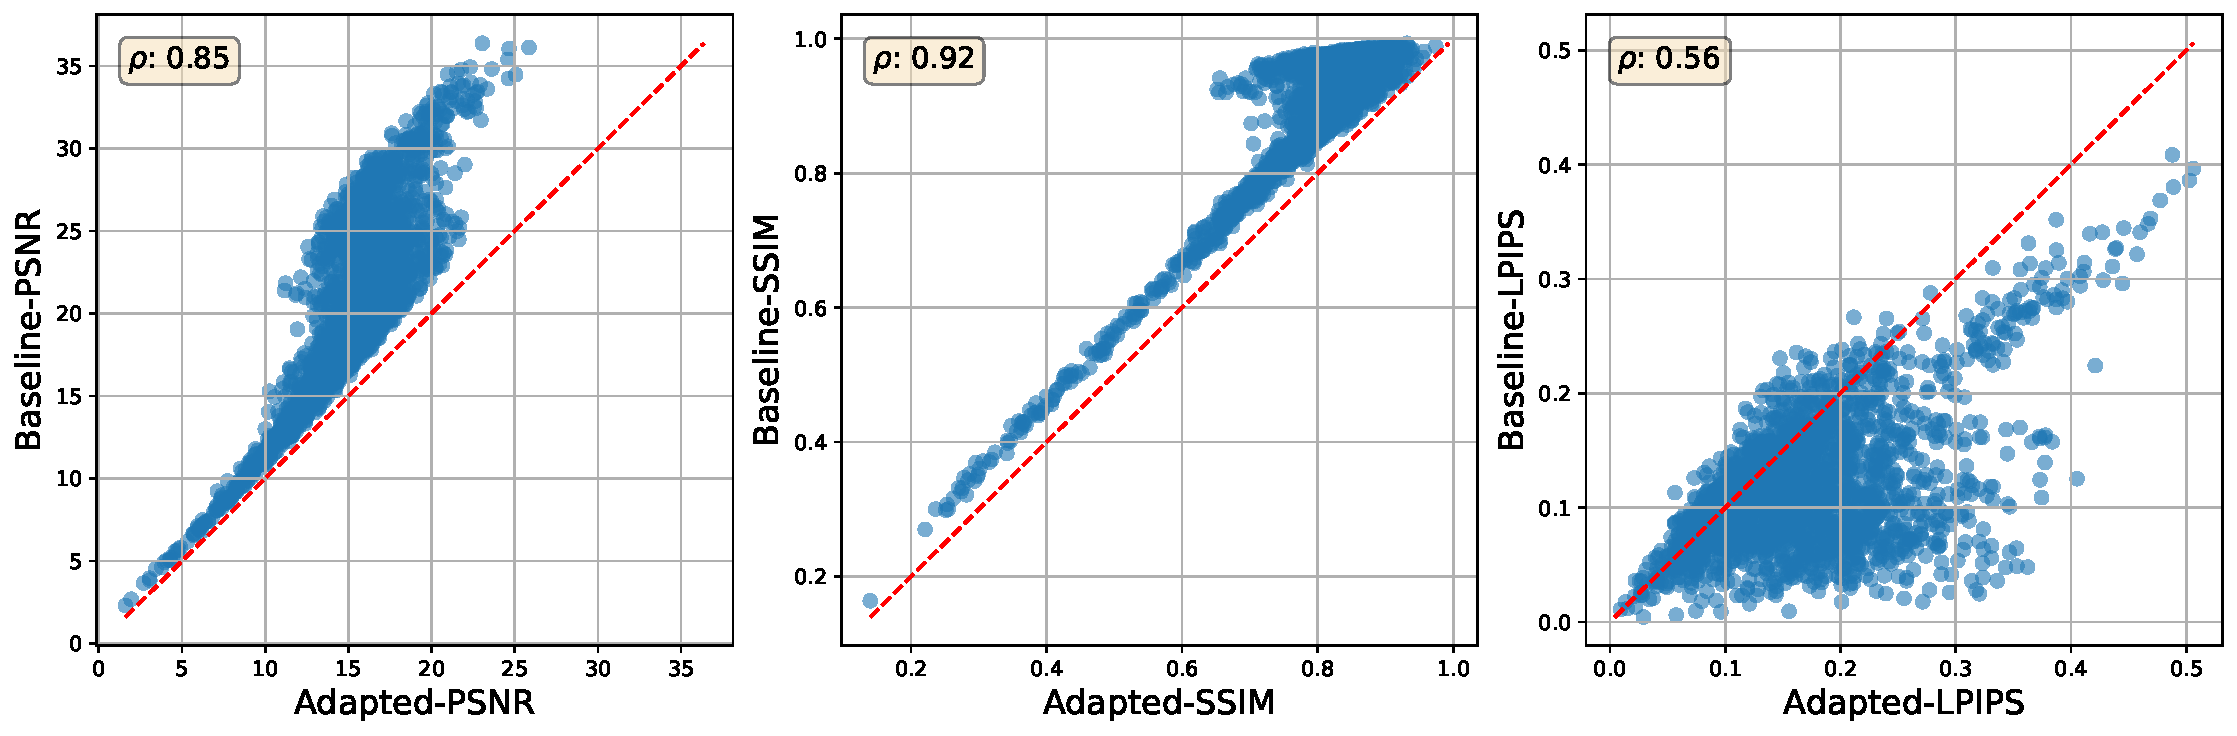
\includegraphics[scale=0.38]{Includes/5-target-prediction-with-domain-gap-dataset.pdf}
            \caption{Performance obtained by super resolving the degraded synthetic FOREST images using different super resolution models.}
            \label{fig:5-target-prediction-with-domain-gap-dataset}
        \end{figure}


        In the frequency domain, the results  are shown in Fig. \ref{fig:5-target-prediction-with-domain-gap-fft}.  
        The adapted model adds amplification in the higher range of spatial frequency, related with noise and artifacts. The frequencies related to the proper signal are also amplified, suggesting an improvement in the resolution.
        This suggests that while the adapted model highlights edges and details, it also severly amplifies the noise and artifacts, resulting in a worse performance in terms of PSNR.
        It is important to note that the amplification curve does not show a considerable difference with respect to the one in Fig. \ref{fig:5-target-amplification-statistics},
        highlighting the fact that the frequency analysis is not suitable by itself to evaluate the performance of the SR model.

        \begin{figure}[H]
            \centering
            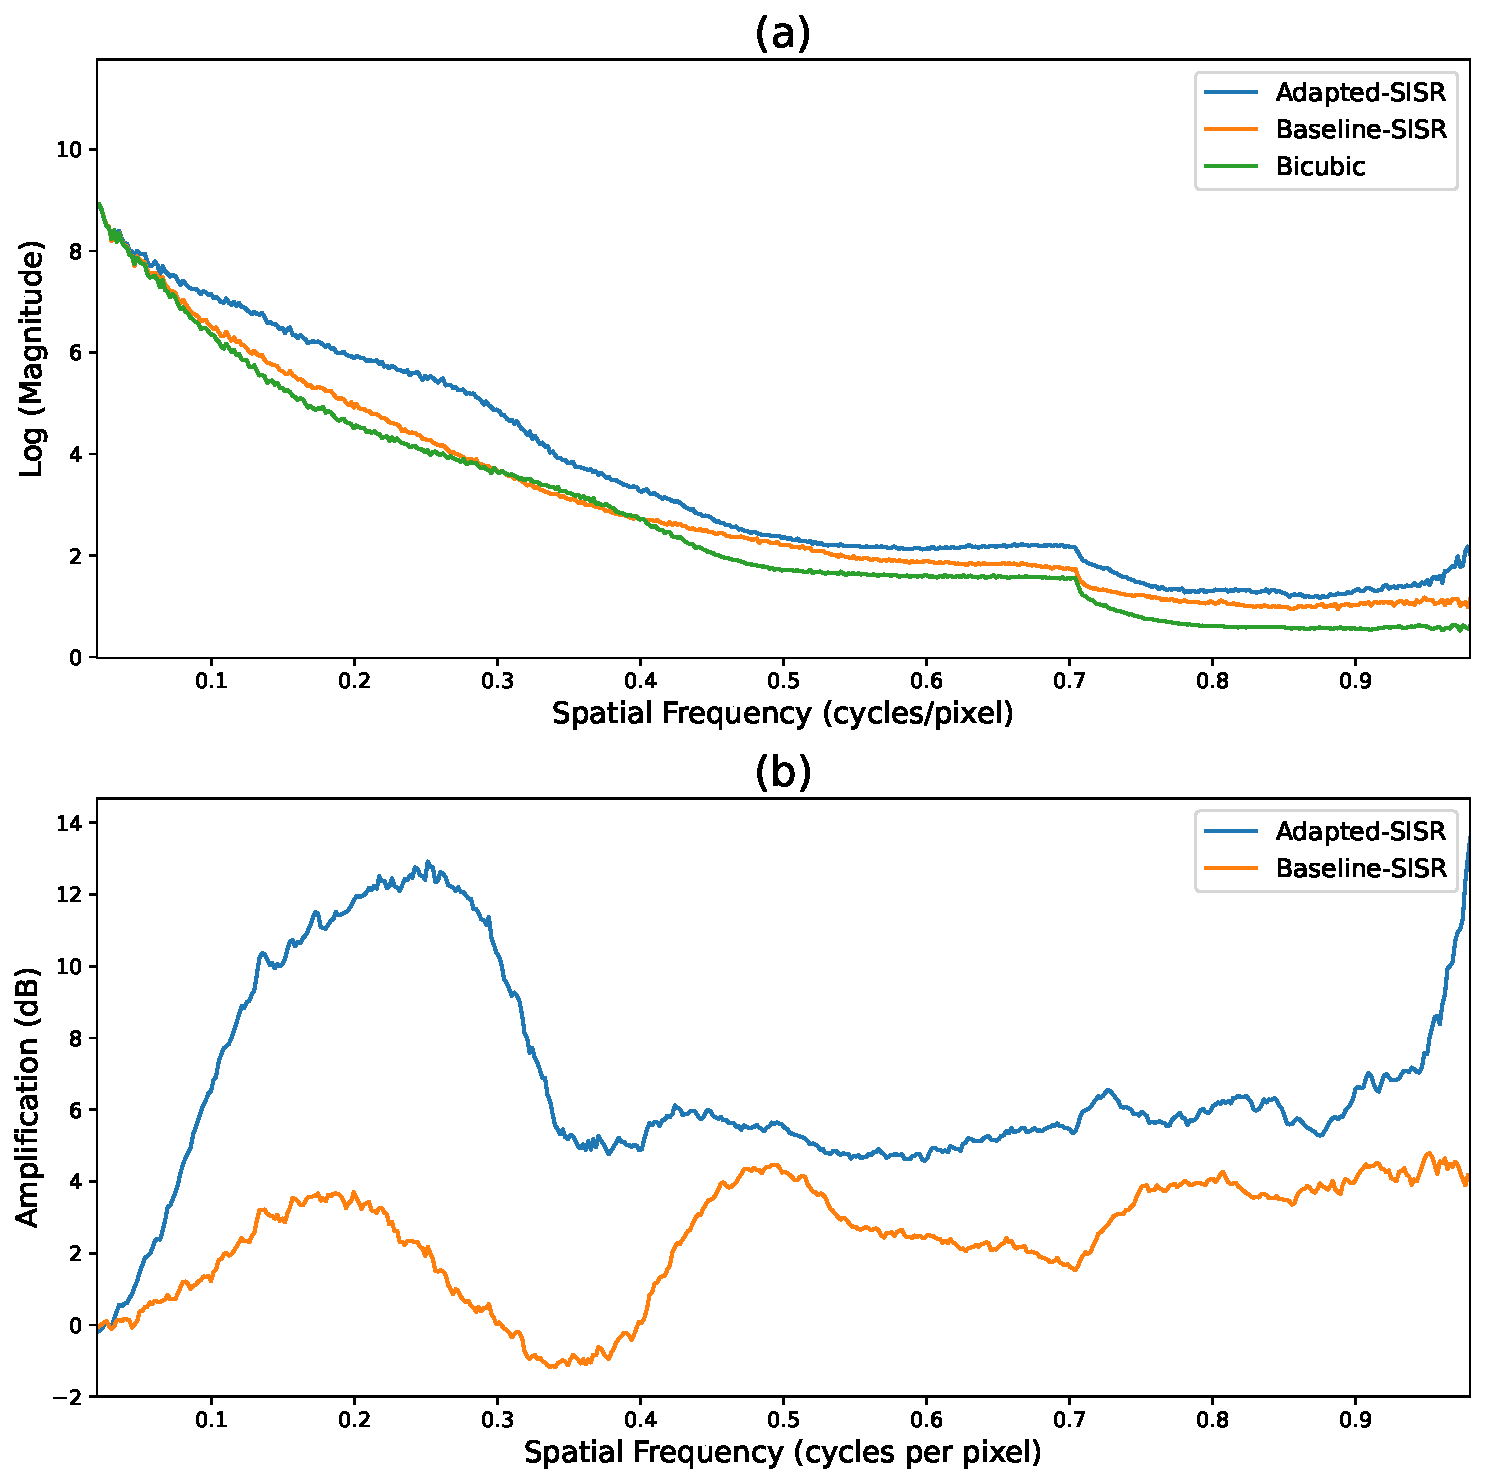
\includegraphics[scale=0.4]{Includes/5-target-prediction-with-domain-gap-fft.pdf}
            \caption{Effects of using a model trained with on different domain than at inference time. 
                     (a) shows the log magnitude of the radial average of the FFT for the SR images using different algorithms.
                     (b) shows the amplification with respect to bicubic interpolation
                     }
            \label{fig:5-target-prediction-with-domain-gap-fft}
        \end{figure}

        
        
    This demonstrates that while this approach is very good to bridge a domain gap, it is not robust at all to domain shifts. 
    This limitation is in sync with what is found in the literature, where GAN approaches are not able to generalize to arbitrary domains DASDASD.


    As in the target domain the ground truth is not known due to the lack of a paired dataset, the performance of the SR model can not be evaluated using metrics like PSNR and SSIM.
    The result of the image quality assessment metrics were done by super resolving images coming from real FOREST-2 and also from the degraded synthetic FOREST-2 images and calculating their NIQE and BRISQUE scores.
    The results are shown in Fig. \ref{fig:5-target-iqa-results}.
    For both metrics, a large gap is observed between the adapted model and the rest, when the input images come from real FOREST-2 images. 
    Suggesting that the adapted model is able to produce more natural images than the rest.
    This behaviour does not exactly replicates when the input images come from synthetic FOREST-2 images, where the adapted model is not able to produce more natural images than the rest.
    Moreover, for the adapted model, both metrics tend to get worse when the input images come from synthetic FOREST-2 images. The contrary happens for the rest of the models.
    This suggests that the adapted model is able to produce more natural images than the rest, but only when the input images come from the same distribution as the target domain used in training.
    However, it is important to note that: 

    \begin{enumerate}
        \item The images used for training the NIQE and BRISQUE models are not remote sensing images, and therefore, the results may not be representative. This could be circumvented by training a NIQE/BRISQUE model using remote sensing images only.
        \item NIQE and BRISQUE are objective measures of image quality, not of physical consistency or image fidelity.
    \end{enumerate}

    While the comparison of results may help to understand the behaviour of the models, it is important to note that the results are not representative of the real world performance of the models. 

        \begin{figure}[H]
            \centering
            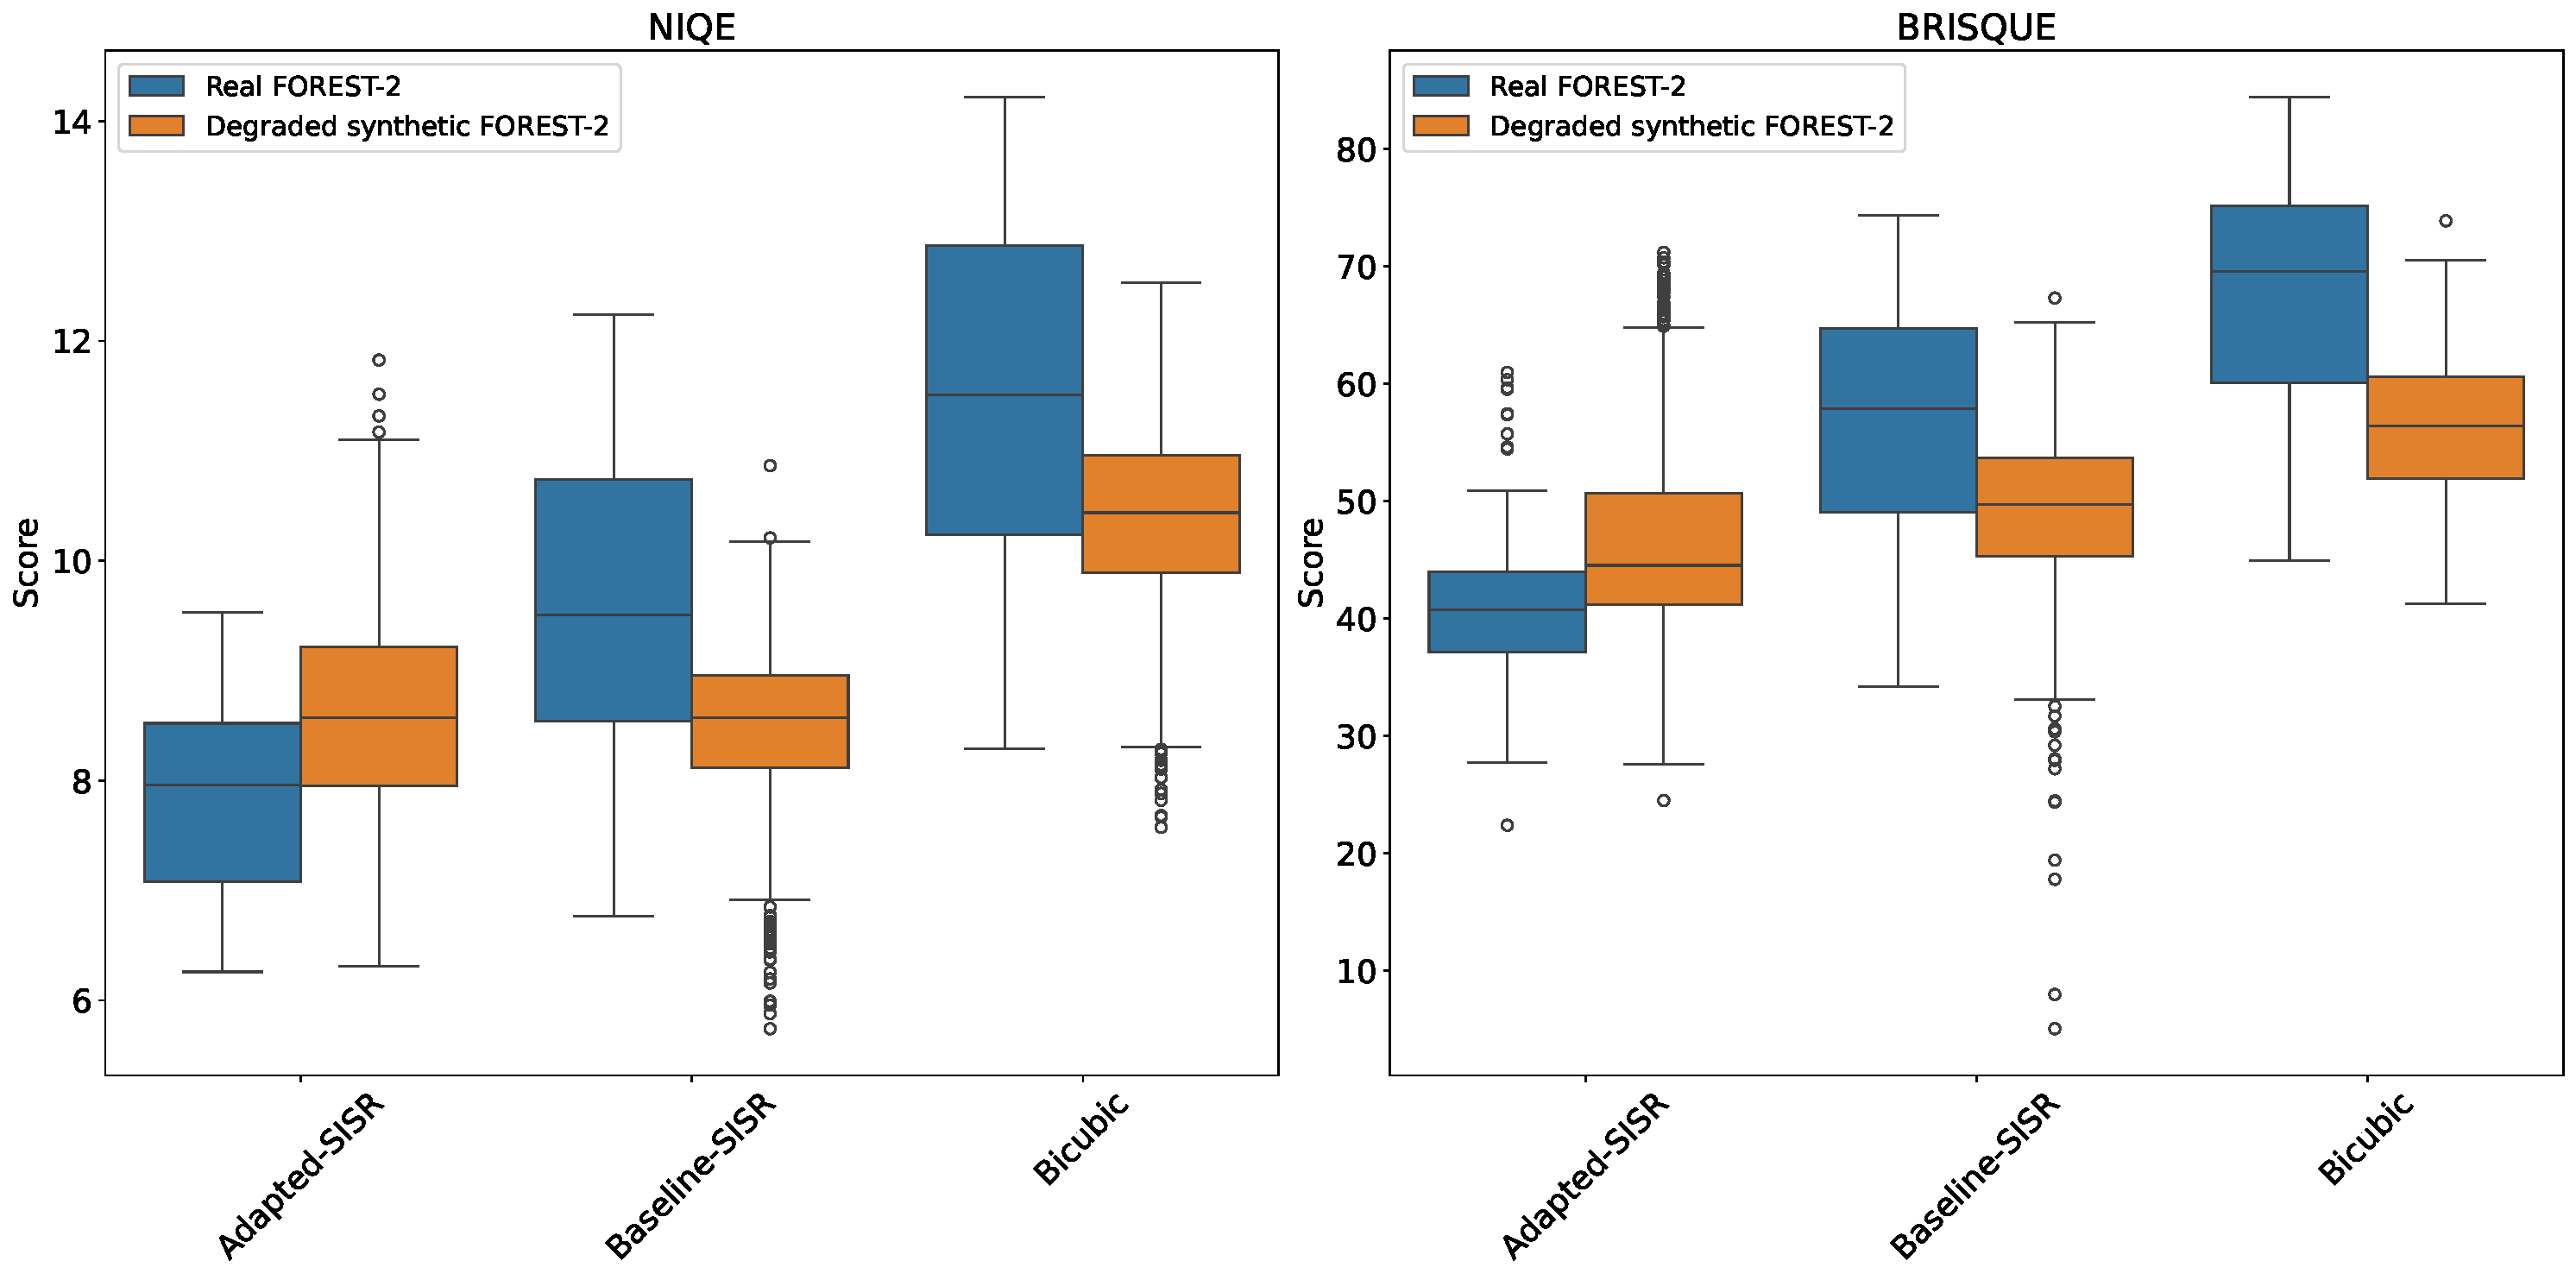
\includegraphics[scale=0.28]{Includes/5-target-iqa-results.pdf}
            \caption{Image quality assessment metrics for the different SR models using different datasets as input. 
                    In both metrics, the lower the score, the better the image quality.}
            \label{fig:5-target-iqa-results}
        \end{figure}


        

        
% \breakpage
    